\documentclass[12pt,a4paper]{article}
\usepackage[utf8]{inputenc}
\usepackage[T1]{fontenc}
\usepackage[ngerman]{babel}
\usepackage{csquotes}
\usepackage[backend=biber,style=authoryear,maxcitenames=2,maxbibnames=99]{biblatex}
\addbibresource{Organisation.bib} % Bib-Datei nicht vergessen!
\newcommand{\zitat}[1]{\parencite{#1}}
\usepackage{geometry}
\geometry{
	left=30mm,
	right=30mm,
	top=25mm,
	bottom=25mm
}
\usepackage{graphicx}
\usepackage{float}
\usepackage{setspace}
\onehalfspacing
\usepackage{caption}
\usepackage{tocloft}
\usepackage{hyperref}
\hypersetup{colorlinks=true, linkcolor=black, urlcolor=blue, citecolor=black}
\usepackage{acronym}
\usepackage[nottoc]{tocbibind}
\usepackage{etoolbox} % für robusten Befehl
\usepackage{lipsum} % nur für Blindtext, kann entfernt werden
\usepackage{setspace} % für Zeilenabstand
\usepackage{ragged2e} % für \justifying





\newcommand{\absatzZitat}[1]{%
	\begin{quote}
		\fontsize{10pt}{12pt}\selectfont
		\setstretch{1.0}
		\leftskip=1cm
		\rightskip=1cm
		\justifying
		#1
	\end{quote}
}

\begin{document}
	
	%------------------------- Titelseite -------------------------
	\begin{titlepage}
		\centering
		\vfill
		{\Huge \textbf{Deutsche Telekom}}\\[1.5cm]
		\large
		Seminar: Grundlagen der Organisation\\
		Sommersemester 2025\\[2cm]
		
\includegraphics[width=0.4\textwidth]{images/UOL-Logo.png}\\[2cm]
		\normalsize
		\begin{flushleft}
			\textbf{Betreurin:} Prof. Dr. Julia Brennecke\\[0.5cm]
			\textbf{Abgegeben von:}\\
			Mika Scheinig\\
			Elija Wendte\\
			Justus Kressmann\\
			Engin Fidansoy\\
			Manar Krenbeh\\[0.5cm]
			Carl von Ossietzky Universität Oldenburg\\
			Fakultät II – Informatik, Wirtschafts- und Rechtswissenschaften\\
		\end{flushleft}
		\vfill
		\begin{flushright}
			Abgabedatum: 01. Juni 2025
		\end{flushright}
	\end{titlepage}
	
	%------------------------- Eidesstattliche Erklärung -------------------------
	\pagenumbering{Roman}
	
	\section*{\texorpdfstring{Executive Summary}{Executive Summary }}\label{executive-summary}
	
	In diesem Bericht wird die Aufbau- und Ablauforganisation der Deutschen
	Telekom AG untersucht, die mit rund 200.000 Mitarbeitenden in mehr als
	50 Ländern zu den größten Telekommunikationsanbietern weltweit gehört.
	Der Konzern organisiert sich im Wesentlichen divisional, wobei
	Matrixelemente in Bereichen wie IT, Personal und Strategie hinzukommen.
	Diese hybride Struktur soll Spezialisierung, Kund:innennähe und
	Flexibilität ermöglichen. Allerdings ergeben sich dabei auch
	Schwierigkeiten bei Koordination, Abstimmung und der Bestimmung
	eindeutiger Zuständigkeiten. Die Analyse legt offen, dass interne
	Abläufe teils als schwerfällig wahrgenommen werden.
	Entscheidungsprozesse nehmen viel Zeit in Anspruch, interdisziplinäre
	Kooperation funktioniert nicht optimal, und Silo-Denken erschwert eine
	übergreifende Sichtweise. Agile Arbeitsformen lassen sich unter diesen
	Bedingungen schwer integrieren. Bestehende Initiativen wie digitale
	Lernplattformen, neue Führungsmodelle und bereichsübergreifende Projekte
	sind wichtige Schritte, reichen jedoch nicht aus, um strukturelle
	Schwächen zu beheben.
	
	\noindent Der Schwerpunkt liegt auf der Geschäftseinheit T-Systems, bei der ein
	gesteigerter Veränderungsbedarf festgestellt wurde. Die Analyse zeigt
	Potenziale in Effizienz, Zuständigkeiten und Kulturentwicklung. Erste
	Handlungsideen wie klare Schnittstellen, effizientere Prozesse und
	vernetzte Zusammenarbeit werden skizziert. Der Bericht bildet die Basis
	für einen Folgebericht mit konkreten Empfehlungen zur Reorganisation von
	T-Systems.
	
	
	%------------------------- Inhaltsverzeichnis -------------------------
	\newpage
	\tableofcontents
	\newpage
	
	%------------------------- Abbildungsverzeichnis -------------------------
	\listoffigures
	\newpage
	
	%------------------------- Tabellenverzeichnis -------------------------
	\listoftables
	\newpage
	
	%------------------------- Abkürzungsverzeichnis -------------------------
	\section*{Abkürzungsverzeichnis}
	\begin{acronym}[IT]
		\acro{IT}{Informationstechnologie}
		\acro{BWL}{Betriebswirtschaftslehre}
	\end{acronym}
	\newpage
	
	%------------------------- Kapitelstruktur -------------------------
	
	\pagenumbering{arabic}
	\setcounter{page}{1}
	\begin{center}
		\textbf{Report 1 – Deutsche Telekom}
	\end{center}
	
	
	
	\section{Einleitung und Unternehmensvorstellung}
	
	\subsection{Kontext und Relevanz}
	Warum wurde diese Organisationseinheit gewählt?
	
	Einordnung in das Unternehmen (z.B. Bereich, Funktion, strategische Bedeutung)
	
	\subsection{ Überblick zur Organisationseinheit}
	Größe, Struktur, Aufgabenbereich
	
	Rolle innerhalb des Gesamtunternehmens
	\subsection{Kontext und Relevanz}
	Was soll mit dem Bericht erreicht werden?
	
	Kurze Vorschau auf den inhaltlichen Aufbau
	
	\subsection{Zielsetzung der Analyse}
	Was soll mit dem Bericht erreicht werden?
	
	Kurze Vorschau auf den inhaltlichen Aufbau
	
	
	\section{Analyse der informellen Organisation}
	\subsection{Informelle Strukturen und kulturelle Merkmale}
	Werte, Normen, interne Denkweisen
	
	Machtverhältnisse, Netzwerkstrukturen
	
	Informelle Kommunikation und Entscheidungswege
	\subsection{Elemente moderner Organisationsformen}
	Einsatz von agilen Methoden, selbstorganisierten Teams etc.
	
	Technologische Infrastruktur (z.B. Tools, Plattformen)
	
	Zusammenarbeit über Bereichsgrenzen hinweg (Cross-Functional Work)
	\subsection{Identifizierte Herausforderungen}
	
	Welche Spannungen oder Schwächen ergeben sich aus der Analyse?
	
	Konkrete Pain Points mit Bezug zur Organisationseinheit
	
	Bezug zur Risikoanalyse aus dem Geschäftsbericht
	
	\section{Entwicklung eines Konzepts für organisationalen Wandel}
	Im Folgenden wird aufbauend auf den zuvor identifizierten Herausforderungen ein Konzept entwickelt, das gezielt auf die Förderung organisationaler Agilität und Anpassungsfähigkeit abzielt. Ziel ist es, die bestehenden internen Schwächen im Entscheidungsverhalten, der Zusammenarbeit und Reaktionsgeschwindigkeit durch geeignete strukturelle, technologische und kulturelle Maßnahmen zu adressieren.
	
	\noindent Die Darstellung erfolgt entlang von fünf Teilaspekten: Zunächst wird der konkrete Problemfokus skizziert, anschließend werden Zielsetzung, zentrale Maßnahmen, der Umgang mit Widerständen sowie erforderliche Rahmenbedingungen ausgearbeitet.
	\subsection{Ausgangspunkt und Problemfokus}
	
	Auf Grundlage der vorangegangenen Analyse zeigt sich als besonders gravierendes Problem die unzureichende Agilität der internen Organisation. Diese äußert sich unter anderem in langsamen Entscheidungsprozessen, fehlender bereichsübergreifender Abstimmung und einer eingeschränkten Anpassungsfähigkeit an technologische, regulatorische und marktbezogene Veränderungen. Damit verbunden ist eine hohe Belastung für Mitarbeitende, eine erschwerte Integration technologischer Systeme sowie ein erhöhter Koordinationsaufwand im internationalen Wettbewerb. Diese Faktoren wirken sich direkt auf die Innovationsfähigkeit, Umsetzungsstärke und Wettbewerbsposition der Organisation aus.
	
	\noindent Das folgende Konzept setzt an diesem Pain Point an und entwickelt konkrete Lösungsansätze, die auf vier zentralen Wirkfeldern aufbauen: der Förderung organisationaler Agilität, dem gezielten Einsatz von Cloud-Technologien und SaaS-Lösungen, der Stärkung von Wissensmanagement und HR-Strukturen sowie dem strategischen Einsatz von Business Intelligence zur Entscheidungsunterstützung. Die Maßnahmen orientieren sich an den im Geschäftsbericht 2021 benannten Risikofeldern wie z.\,B. technologischer Abhängigkeit, Integrationsproblemen, Fachkräftemangel und regulatorischem Druck.
	
	\noindent Abschließend werden Handlungsempfehlungen formuliert, die darauf abzielen, das Konzept unternehmensintern anschlussfähig zu machen – insbesondere vor dem Hintergrund möglicher personeller und struktureller Widerstände gegenüber Veränderungen. Dabei werden sowohl personenbezogene Ursachen wie Unsicherheit, Statusängste oder fehlendes Verständnis, als auch organisationsbezogene Faktoren wie bestehende Anreizsysteme oder Machtstrukturen berücksichtigt \parencite{schmelzerHermannJ2020GidP}.
	
	
\subsection{Zielsetzung des Konzepts}

Das übergeordnete Ziel des vorliegenden Konzepts besteht darin, die organisationale Agilität innerhalb der betrachteten Organisationseinheit der Deutschen Telekom gezielt zu stärken. Hierzu sollen strukturelle, technologische und kulturelle Voraussetzungen geschaffen werden, die eine schnellere, koordinierte und flexiblere Reaktion auf externe Anforderungen ermöglichen.

\noindent Die Zielsetzung folgt dem in der strategischen Zielplanung etablierten System aus Sach- und Formalzielen \parencite{StelzerDirk1962-2011I:GA}. Im Zentrum stehen folgende Zielinhalte:

\begin{itemize}
	\item \textbf{Sachziel:} Erhöhung der Anpassungsfähigkeit der Organisation an regulatorische, technologische und marktbezogene Veränderungen durch den gezielten Einsatz agiler Arbeitsformen, cloudbasierter Informationssysteme und strukturierter Wissensprozesse.
\item \textbf{Formalziele:}
\begin{itemize}
	\item \textit{Wirksamkeitsstreben:} Durch die Einführung klarer Entscheidungsprozesse, digitaler Abstimmungswerkzeuge und fester Zuständigkeiten soll die Entscheidungsfindung nachvollziehbar und effizient gestaltet werden.
	
	\item \textit{Anpassungsstreben:} Durch den Einsatz agiler Arbeitsmethoden, modularer Prozessbausteine und flexibler Teamstrukturen sollen Veränderungen kontinuierlich und ohne tiefgreifende Systembrüche umgesetzt werden.
	
	\item \textit{Wirtschaftlichkeitsstreben:} Durch die Nutzung vorhandener IT-Systeme, die Weiterqualifizierung bestehender Mitarbeitender und eine schrittweise Implementierung der Maßnahmen sollen Ressourcen geschont und Kosten gering gehalten werden.
\end{itemize}
\end{itemize}



\subsection{Zielsystem}

Innerhalb von zwölf Monaten soll die durchschnittliche Dauer für bereichsübergreifende Entscheidungsprozesse um mindestens 30\,\% reduziert werden, gemessen in Tagen vom Antrag bis zur Umsetzung.

\noindent Der Anteil von Projekten, an denen Mitarbeitende aus mindestens zwei unterschiedlichen Bereichen beteiligt sind, soll im selben Zeitraum um 20\,\% steigen; Grundlage ist die Auswertung interner Projektberichte.

\noindent Die Zustimmung zur Aussage „Veränderungen werden klar und nachvollziehbar kommuniziert“ soll in einer internen Umfrage nach sechs Monaten mindestens 75\,\% betragen, gemessen über eine standardisierte Zufriedenheitsabfrage.

\noindent Die Zahl der Nachsteuerungen bei umgesetzten Entscheidungen soll innerhalb eines Jahres um 25\,\% gesenkt werden, gemessen anhand dokumentierter Rückläufer oder Überarbeitungen im Projektcontrolling.


\noindent Die formulierten Ziele schaffen eine klare Orientierung für die Umsetzung des Konzepts und bilden zugleich die Grundlage für eine kontinuierliche Überprüfung und Steuerung der angestrebten Veränderungen.

\noindent Die Zielerreichung wird durch definierte Teilmaßnahmen, Indikatoren und einen konkreten zeitlichen Umsetzungsrahmen operationalisiert. Eine Bewertung erfolgt u.\,a. anhand von KPIs wie Durchlaufzeiten für Entscheidungen, Beteiligung interdisziplinärer Teams an Innovationsprozessen und Rückmeldungen aus dem internen Change-Feedback.


	\subsection{Konzeptionelle Ansätze und Maßnahmen}
	
	\subsection{BI-gestützte Entscheidungsarchitektur zur Stärkung der Agilität}
	
	Basierend auf den Erkenntnissen von Smith und Ariyachandra (2021) lässt sich ein Konzept ableiten, das den gezielten Einsatz von Business Intelligence (BI) zur Verbesserung von Entscheidungsprozessen innerhalb der Deutschen Telekom vorsieht. Die zentralen Herausforderungen bei FEMA – insbesondere die mangelnde Datenintegration, fehleranfällige Prozesse und unklare Verantwortlichkeiten – sind auch in komplexen Konzernen wie der Telekom in ähnlicher Form beobachtbar, etwa in Form langwieriger Entscheidungswege und fehlender Transparenz über bereichsübergreifende Vorgänge.
	
	Das FEMA-Projekt zeigt exemplarisch, wie eine einfache, aber strukturierte BI-Lösung zu mehr Agilität, Kontrolle und Effizienz führen kann. Durch die Zusammenführung dezentraler Datenquellen, automatisierte Validierungslogiken und rollenbasiertes Reporting konnte innerhalb kurzer Zeit ein transparentes Entscheidungsfundament geschaffen werden. Die Autoren betonen: „A simple integrated BI solution […] can vastly enhance the post disaster operations […] and improve its agility during humanitarian crises“ \parencite[S.~210]{smithAriyachandra2021}.
	
	Übertragen auf die Telekom ergibt sich folgende methodische Vorgehensweise:
	
	\begin{itemize}
		\item \textbf{1. Datenerfassung und -bereinigung:} Aufbau eines automatisierten Validierungsprozesses zur Sicherung der Datenqualität aus verschiedenen operativen Systemen. „Data accuracy and data completeness are among some of the key data quality problems that plague BI and analytics projects“ \parencite[S.~201]{smithAriyachandra2021}.
		
		\item \textbf{2. Integration in ein zentrales Entscheidungsdatenmodell:} Aufbau einer modularen, cloud-basierten BI-Infrastruktur mit klar definierten Schnittstellen zu allen beteiligten Bereichen. Ziel ist ein einheitliches, strukturiertes Datenmodell für bereichsübergreifende Steuerung.
		
		\item \textbf{3. Rollenbasiertes Echtzeit-Reporting:} Einführung von Dashboards und interaktiven Analyseoberflächen, die relevante Entscheidungskennzahlen nach Verantwortungsbereich aufbereiten (z.\,B. Zeit bis zur Entscheidung, Anzahl Rückläufe, Beteiligungsintensität). Dies entspricht der Idee, dass „BI empowers frontline users […] for more effective decision making“ \parencite[S.~201]{smithAriyachandra2021}.
		
		\item \textbf{4. Governance und Verantwortlichkeiten:} Einführung eines zentralen BI-Governance-Modells mit klaren Zuständigkeiten für Datenqualität, Analysezugriff und KPI-Verantwortung. Denn: „The lack of centralized governance structures and practices“ war laut der Autoren ein zentrales Hemmnis für agile Entscheidungsfindung bei FEMA \parencite[S.~208]{smithAriyachandra2021}.
		
		\item \textbf{5. Pilotierung mit agilen Teams:} Um kulturelle und strukturelle Barrieren schrittweise abzubauen, sollte das System zunächst in ausgewählten interdisziplinären Teams getestet werden, bevor eine skalierte Ausweitung erfolgt. So können Widerstände frühzeitig identifiziert und adressiert werden.
	\end{itemize}
	
	Dieses Konzept zielt darauf ab, Entscheidungsprozesse nicht nur zu beschleunigen, sondern auch robuster, nachvollziehbarer und datengestützt zu gestalten – ein zentraler Hebel, um die organisationale Agilität im Sinne der übergeordneten Zielsetzung nachhaltig zu verbessern.
\subsection{Ergänzende Perspektive: SaaS als strategischer Enabler für agile Entscheidungsarchitekturen}

Ergänzend zur BI-orientierten Perspektive auf datenbasierte Entscheidungsfindung eröffnet die strategische Migration zu Software-as-a-Service (SaaS) ein zusätzliches Handlungsfeld: Während Business Intelligence die analytische Seite von Entscheidungen adressiert, ermöglicht SaaS die strukturelle und technologische Flexibilisierung der zugrundeliegenden Prozesse selbst. Insbesondere für Konzerne wie die Deutsche Telekom, deren Entscheidungsarchitekturen über viele organisatorische Ebenen verteilt sind, kann der SaaS-Ansatz als Hebel zur Reduktion von Komplexität und zur Stärkung bereichsübergreifender Abstimmung dienen.

Die Einführung von SaaS in Entscheidungsprozesse lässt sich dabei als gestufte Transformation denken. Basierend auf dem Reifegradmodell von Kang et al. (2008) sowie Churakova und Mikharamova (2010), empfiehlt sich ein inkrementelles Vorgehen: Beginnend mit der Entkopplung zentraler Datenbanken („DB on Cloud“) und der Virtualisierung bestehender Entscheidungsräume („Virtual System Space“), können mittelfristig serviceorientierte Prozessbausteine („Full SOA“) etabliert und langfristig maßgeschneiderte SLA-basierte Workflows („Custom App/SLA“) eingeführt werden. Diese Entwicklung führt nicht nur zu einer technologischen Modernisierung, sondern fördert auch die Transparenz und Steuerbarkeit von Entscheidungen auf allen Ebenen.

Ein besonderer Vorteil ergibt sich durch die Möglichkeit, Entscheidungsprozesse softwaregestützt modular zu definieren, zentral zu überwachen und kontinuierlich anzupassen. Wie im FEMA-Fall gezeigt, ist gerade diese Flexibilität entscheidend: „Cloud-based knowledge management […] provides the agility it requires to provide high quality experiences to customers and service delivery“ \parencite[S.~58]{churakova2020}. Übertragen auf die Telekom bedeutet das: Entscheidungen werden nicht länger an starre Abläufe gebunden, sondern können entlang definierter Services dynamisch orchestriert werden – mit klaren Verantwortlichkeiten, Echtzeit-Feedback und technischer Skalierbarkeit.

Diese Architektur zahlt direkt auf die zuvor definierten Formalziele ein: Sie steigert die Wirksamkeit, indem Entscheidungswege nachvollziehbar und responsiv gestaltet werden; sie stärkt die Anpassungsfähigkeit, indem neue regulatorische oder marktbezogene Anforderungen durch konfigurierbare Services abgebildet werden können; und sie erhöht die Wirtschaftlichkeit, da zentrale Dienste einmal entwickelt und vielfach genutzt werden können – auch über Bereichsgrenzen hinweg.

Durch die Kombination von BI-basierter Entscheidungsunterstützung und SaaS-gestützter Entscheidungsstruktur entsteht ein ganzheitliches Konzept zur Stärkung organisationaler Agilität, das sowohl auf technologische als auch auf prozessuale Hebel zurückgreift.
	
	
	
	Strukturelle Maßnahmen
	z.B. Einführung agiler Teams, Cross-Functional Units, flachere Hierarchien
	
	Technologische Maßnahmen
	z.B. SaaS-Implementierung, digitale Plattformen zur Zusammenarbeit
	
	Kulturelle Maßnahmen
	z.B. Förderung kollektiver Intelligenz, Dialogformate, Innovationsräume
	
	(Optional) Kurze Visualisierung oder Tabelle zur Übersicht
	\subsection{Umgang mit potenziellen Widerständen}
	Bezug auf bekannte Widerstandsursachen (vgl. Abbildung)
	
	Maßnahmen zur Förderung der Akzeptanz:
	
	Partizipation
	
	Change Agents
	
	Kommunikation und Transparenz
	
	Weiterbildung
	
	Ziel: Konzept so gestalten, dass es nicht gegen, sondern mit den Mitarbeitenden umgesetzt wird
	
	\subsection{Voraussetzungen und Erfolgsfaktoren}
	Was braucht es, damit das Konzept funktioniert?
	→ z.B. Unterstützung durch Führung, Ressourcen, Pilotbereiche
	
	Verbindung zu bestehenden Initiativen in der Organisation (z.B. Tech  Innovation bei der Telekom)
	
	\section{Diskussion der Ergebnisse}
	\subsection{Bewertung der vorgeschlagenen Maßnahmen}
	
	Was leisten die Maßnahmen im Hinblick auf die analysierten Probleme?
	Welche Verbesserungen wären zu erwarten?
	\subsection{Potenziale und Chancen}
	Welche Entwicklungsmöglichkeiten ergeben sich für die Organisationseinheit?
	
	Langfristiger Nutzen (z.B. Innovationskraft, Arbeitgeberattraktivität)
	\subsection{Risiken und Grenzen}
	Was könnte die Umsetzung erschweren? (z.B. Ressourcen, Akzeptanz, Führung)
	
	Wo stößt das Konzept an Grenzen?
	
	\subsection{Einschätzung zur Umsetzbarkeit}
	Was spricht für die praktische Umsetzung?
	
	Welche Voraussetzungen müssen erfüllt sein?
	%------------------------- Literaturverzeichnis -------------------------
	
	\newpage
	\pagenumbering{roman}
	\printbibliography[heading=bibintoc,title={Literaturverzeichnis}]
	
	
	%------------------------- unternehmensinfo -------------------------
	\newpage
	\thispagestyle{empty} % keine Seitenzahl anzeigen
	\begin{figure}[H]
		\centering
		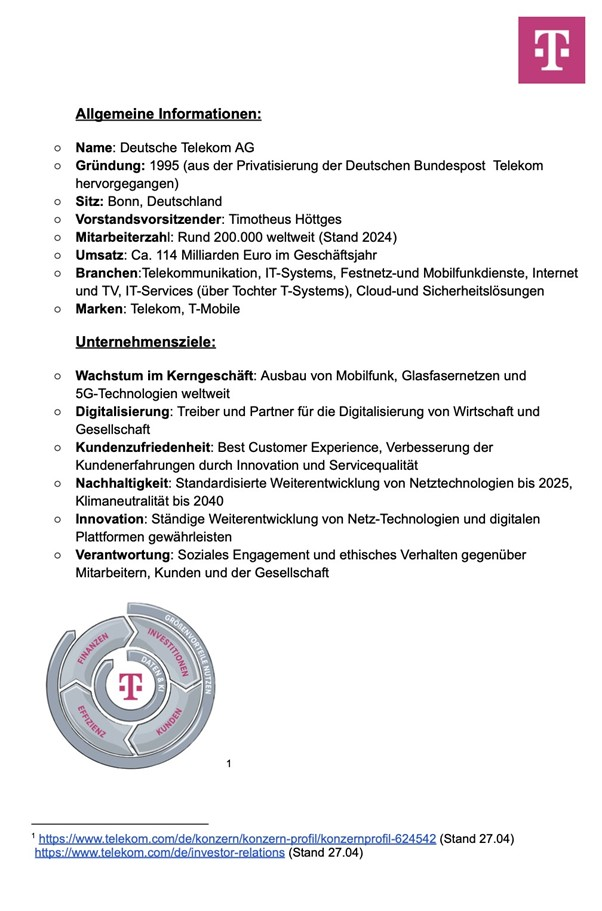
\includegraphics{images/Bild1.jpg}
	\end{figure}
	\newpage
	%------------------------- Anhang -------------------------
	\newpage
	\section{Anhang}
	[Zusätzliche Materialien wie Interviewleitfäden etc.]
	
	%------------------------- KI-Nutzung -------------------------
	\newpage
	\section{Anhang: Nutzung von Künstlicher Intelligenz}
	\begin{itemize}
		\item \textbf{Tool:} ChatGPT
		\item \textbf{URL:} \url{https://chatgpt.com}
		\item \textbf{Prompt:} „Erstelle eine vollständige LaTeX-Vorlage für eine Gruppenarbeit.“
		\item \textbf{Verwendet durch:} Mika Scheinig, Elija Wendte, Justus Kressmann, Engin Fidansoy, Manar Krenbeh
		\item \textbf{Datum:} 04.07.2025
	\end{itemize}
	\begin{itemize}
		\item \textbf{URL:} \url{https://chatgpt.com/share/682f2a68-37b8-8007-9855-d878bcd54ae3}
		\item \textbf{Prompt:} „Kannst du mir ein konkretes Beispiel für einen überregulierten internen Prozess der Deutschen Telekom nennen?“
		\item \textbf{Verwendet durch:} Mika Scheinig
		\item \textbf{Datum:} 22.05.2025
	\end{itemize}
	
	\begin{itemize}
		\item \textbf{URL:} \url{https://chatgpt.com/c/683721e2-4a9c-8001-b0a1-f2e5a1b3f5f2}
		\item \textbf{Prompt:} „Bitte erläutere die Unterschiede in der Leitungsspanne zwischen standardisierten operativen Bereichen und komplexeren Organisationseinheiten wie der Matrixorganisation bei T-Systems. Wie beeinflusst die Organisationsstruktur die Anzahl der direkt unterstellten Mitarbeitenden, und welche Herausforderungen ergeben sich für Führungskräfte in einer Matrixstruktur?“
		\item \textbf{Verwendet durch:} Justus Kressmann
		\item \textbf{Datum:} 24.05.2025
	\end{itemize}
	
	\newpage
	\section*{Eidesstattliche Erklärung}
	Hiermit versichern wir, dass wir die vorliegende Arbeit selbstständig und nur mit den angegebenen Hilfsmitteln und Quellen angefertigt haben. Alle Stellen, die wörtlich oder sinngemäß aus Quellen übernommen wurden, sind entsprechend kenntlich gemacht. Die Arbeit wurde in gemeinsamer Verantwortung erstellt.
	
	\vspace{2cm}
	Oldenburg, 01. Juni 2025
	
	Unterschriften: \\
	\rule{5cm}{0.4pt} Mika Scheinig \\
	\rule{5cm}{0.4pt} Elija Wendte \\
	\rule{5cm}{0.4pt} Justus Kressmann \\
	\rule{5cm}{0.4pt} Engin Fidansoy \\
	\rule{5cm}{0.4pt} Manar Krenbeh
	
\end{document}
